%%%% ijcai19.tex

\typeout{IJCAI-19 Instructions for Authors}

% These are the instructions for authors for IJCAI-19.
\documentclass{article}
\pdfpagewidth=8.5in
\pdfpageheight=11in
% The file ijcai19.sty is NOT the same than previous years'
\usepackage{ijcai19}

% Use the postscript times font!
\usepackage{times}
\usepackage{soul}
\usepackage{url}
% \usepackage[hidelinks]{hyperref}
\usepackage[utf8]{inputenc}
\usepackage[small]{caption}
\usepackage{graphicx}
\usepackage{amsmath}
\usepackage{booktabs}
\usepackage{algorithm}
\usepackage{algorithmic}
\urlstyle{same}

\title{Rule Learning}

% Single author syntax
\author{
	Hong Wu, Kewen Wang
	\affiliations
	College of Intelligence and Computing, Tianjin University, China \emails
	wh0625@tju.edu.cn, k.wang@griffith.edu.au
}

\begin{document}
	\maketitle
	
	\begin{abstract}
		% Need to submit before 20:00, February 20, 2019.
		Our work focuses on mining closed-path rules of first order rules from large Knowledge Graphs (KGs). Based on the previous related work, we propose an improved rule learning system with a simplified method of rule search and a novel  paremeter learning model of evaluation. The employment of vector calculation greatly contributed to the scalability of our approach. 
		Since uncertain knowledge graphs have attracted the attention of more researchers, we have tried to transfer the rule learning into the Uncertain Knowledge Graphs (UKGs) using the TensorLog operation. 
		Experiments are conducted on three benchmarks of deterministic KGs and two real-word uncertain KGs via the task of rule mining. The results show that the improvements make the system more scalable, can handle large KGs more efficiently and mine more quality rules, and finally can be applied to the UKG successfully.
	\end{abstract}
	
	
	\section{Introduction}
	With the popularity of {\em Knowledge Garphs (KGs)}, it is widely uesd in various fields, suh as  intelligent web search, QA, advertising recommendation, social media relationship mining, biomedicine, etc. 
	However, the huge amount of data makes it more difficult to construct or complete knowledge graphs manually or automatically.
	How to efficiently process large-scale KGs which contain abundant information and great value, and obtain valuable knowledge related to concerns, are the important issues to be solved urgently.
	
	Typically, knowledge garphs are constructed based on RDF triples. However, the sparse or dense facts surrounding an entity or a relationship are not sufficient to embody the pattern or amount of information in the context of big data.
	Rules are different from the triple form of KGs. It is a higher level abstract pattern representation. The laws they describe can help us better understand the data. It can make use of the new facts generated by rules to further complete the KGs.Also, it can detect the hidden faults in KBs, or be used to reasoning and so on. 
	
	Therefore, as an upstream research problem in the field of knowledge graphs applications, rule learning has certain research and practical significance.
	
	\subsection{Knowledge Graphs}
	Knowledge graph $K = (E, P , F)$ is a structured semantic knowledge base, which describes concepts and their mutual relationships in the physical world with a symbolic form, where $E, P, F$ are the  sets of entities, predicates, and facts respectively. The basic unit is the triple of fact $f: (e_s, p, e_o)$ which denotes subject entity $e_s$ is related to another object entity $e_o$ by the binary predicate $P$. Entities are connected by relationships to form a network of knowledge structures. In order to facilitate the latter rule representation, we convert a fact representation into $p(e_s, e_o)$ for convenience. 
	There are many KGs for research and business like YAGO~\cite{Yago}, DBpedia~\cite{Dbpedia}, Wikidata~\cite{Wikidata} and Freebase~\cite{Freebase}.
	The huge amount of data, incompleteness, and noise data are all difficulties in its research.
	 
	Compared to deterministic KGs, {\em uncertain knowledge graphs} (UKGs) provide a confidence score along with every fact. The development of relation extraction and crowdsourcing in recent years enabled the construction of large-scale uncertain knowledge bases. 
	ConceptNet~\cite{Conceptnet} is a multilingual uncertain KG for commonsense knowledge that is collected through crowdsourcing. The confidence scores in ConceptNet mainly come from the co-occurrence frequency of the labels in crowdsourced task results. 
	NELL~\cite{NELL} collects facts by crawling data of web pages and learns the confidence scores from semi-supervised learning with the Expectation-Maximum (EM) algorithm. 
	The research of uncertain knowledge graph will progress many knowledge-driven applications such as question-answering and intelligent semantic search by providing more uncertain characterization of knowledge.
	
	\subsection{Representation Learning}
	The entities, concepts and relationships in knowledge graphs are represented by discrete and explicit symbols, which are difficult to be directly applied to deep learning models such as neural networks based on continuous numerical representation. 
	In order to effectively utilize the symbolic knowledge in the KGs, researchers have proposed a large number of representation methods for knowledge graphs. These methods transform the entities and predicates of discrete KGs into continuous dimensional space, such as {\bf RESCAL} \cite{Nickel:RESCAL}, {\bf TransE} \cite{Bordes:transe}, {\bf PTransE} \cite{Liu:ptranse} and {\bf DistMult} \cite{Yang:2015}. Deterministic KG embeddings have been extensively explored by recent work. In~\cite{UKG2018}, they propose a novel uncertain KG embedding model {\bf UKGE}, which aims to preserve both structural and uncertainty information of relation facts in the embedding space. 
	
	Based on these embedded representation models, a more reasonable {\em "rule representation"} model can be studied and a rule mining system capable of handling large KG is designed. 
	
	\subsection{Rule Mining}
	\subsubsection{Rule} In this paper, we aim to mine the closed-path rules (CP rules) of the Horn rules. A Horn rule is composed of a head and a body, where the head is a single atom and the body is a set of atoms. An atom is a fact which has variables at the position of subject and object. In Horn rules, CP rules are of the form: 
	\begin{equation} 
	P_1(x, z_1) \wedge P_2(z_1, z_2)... \wedge P_n(z_{n-1}, y) \to P_t(x, y). 
	 \label{eq:cp rule}
	\end{equation}
	Here $P_t$ is head predicate, and the other are body predicates. The variables $x, y, z_i$ can be instantiated by entities. For example: $BornIn(x, z) \wedge Country(z, y) \to Nationality(x, y)$, where the lenth of rule is set to 2 ( not include the head atom).
	It should be noted that although the CP rule contains the symbol "$\to$", it has a different meaning from the implication symbol in the {\em First-Order Logic}. We can judge a rule is valid by the head atom of an instantiated rule holds if all body atoms of the instantiated rule appear in the KB. 
	
	This form of rules is called closed-path because the sequence of predicates' variables in the body of rule forms a closed path from the
subject argument to the object of the head target predicate.
Due to the serial path, we factor in the inverse of predicates in order to mine more rules in practice. We also allow recursion in the CP rules, which means the predicate of head can
appear in the body part.
	
	\subsubsection{Inductive Logic Program} 
	Early research on generating CP rules in KBs focused on {\em Inductive Logic Programming (ILP)}  \cite{Muggleton:ILP}, which mine rules by exploring the space of all possible hypotheses (rules). Although ILP is a mature field, it is still difficult to mine logic rules from the knowledge bases. On one hand, KBs are based on the {\em Open World Assumption (OWA)}, which means that the unknown information cannot be used as negative samples. On the other hand, the scalability of these methods are insufficient to handle the large amount of data contained in large KGs. 
	The {\bf AMIE} \cite{Galarraga:AMIE} system based on ILP uses the partial hypothesis of the {\em Partial Completeness Assumption (PCA)} to "guess" the counterexamples for mining rules from the KBs, and the optimized {\bf AMIE+} \cite{Galarraga:AMIE+} proposes strategies such as pruning and approximation to enable the system to exploring the search space more effectively. In addition, {\bf Neural LP}~\cite{Yang:NeuralLP}, {\bf ScaLeKB}~\cite{Chen:ScaLeKB}, {\bf SWARM}~\cite{Molood:SWARM} and other systems have been proposed, but in dealing with large-scale KBs, the efficiency of systems and the number or quality of rules are still the main challenges of the existing systems.
	
	\subsubsection{The Rule Learner Based on Embedding} 
	\cite{Yang:2015} based on the knowledge graphs embedding representation model {\bf DistMult}, the two tasks of link prediction and rule mining are compared with other work for the first time. In the task of rule mining, the score function is calculated by using the predicate matrix operational similarity as the criterion for selecting rules, and the candidate rule queue is obtained. 
	In the rule extraction task, it is only compared with {\em AMIE}, and only applied to the small data set FB15K-401, which is slightly better than {\em AMIE} in terms of mining efficiency and number of rules. 
	
	The latest work {\bf RLvLR} system \cite{Omran:RLvLR} is proposed to solve the scalability of  processing large knowledge graphs. It adopts a new sampling algorithm combined with the embedded representation learning model and two scoring functions: {\em Synonymy} and {\em Co-cocurrency}. 
	It is superior to the current optimal {\bf AMIE+} system, and can mine more high-quality CP rules efficiently. 
	% still need to change!
	But there are still some improvements in the design of algorithm. When the cardinality of data or the number of predicates are in large-scale and the length of rule becomes longer, the search space is disastrously huge. In addition to this, matrix operation is too slow in the evaluation phase, which must reduce the running speed of the system to a certain extent.
	
	
	\section{The Framework of Algorithm}
	% \subsection{Preliminaries}
	% \subsection{Algorithm Introduction}
	Next is our algorithm framework, which is based on the {\bf RLvLR} system. In Algorithm~\ref{alg:algorithm}, there are several differences between them.
	
	For a certain knowledge graph, we randomly select a predicate as the target predicate $P_t$ to mine as many high-quality rules as possible with body's length (the number of predicates in the body part, excluding the head) less than $MaxLen$. The $Degree$ contains two types of metric thresholds for the quality rules $R$ and high quality rules $QR$: $HC$ and $SC$. For distinct embedding models, there are different parameters $EmbParas$. 
	\begin{algorithm}[tb]
		\caption{Learn rules for a KG and a target predicate}
		\label{alg:algorithm}
		\textbf{Input}: a KG $K=\{E, P, F\}$, a predicate $P_t$\\
		\textbf{Parameter}:an integer $MaxLen \geq 2$, and rule degree \\
		$DEGREE = \{ R_{minSC}, R_{minHC}, QR_{minSC}, QR_{minHC}\} $ 
		and parameters list of embedding $EmbParas$\\
		\textbf{Output}: a set $Rule$ of CP rules
		\begin{algorithmic}[1] %[1] enables line numbers
			% The order of the FOR is soooooo important!!!
			\STATE $E_0, P_0, F_0 = \textsf{SampleByPt}(P_t)$
			\FOR{$ 2 \leq len \leq MaxLen$}
			% \STATE $i=(len+1)/2$
			\STATE $K^{'} = \textsf{Sampling}(K, P_t, MaxLen)$
			\STATE $Ent_{emb}, Pre_{emb} =\textsf{Embedding} (K^{'}, EmbParas)$
			\STATE $Candidate = \emptyset$	
			\STATE $Result=$\textsf{RuleSearch}$(K^{'}, P_t, Ent_{emb}, Pre_{emb},len)$
			\STATE Add $Result$ to $Candidate$
			\ENDFOR
		\STATE $Rule=\textsf{EvaluateAndFilter}(Candidate,K,DEGREE)$
		\RETURN $Rule$
		\end{algorithmic}
	\end{algorithm}

	\subsection{Sample}  
	Due to the characteristic of closed-path rules, we can apply the \textsf{Sampling($\cdot$)} algorithm to get a smaller KB $K^{'}=\{E^{'}, P^{'}, F^{'}\}$ that contains all the potential predicates with related entities and facts before working directly on large KB. 
	\begin{figure}
		\centering
		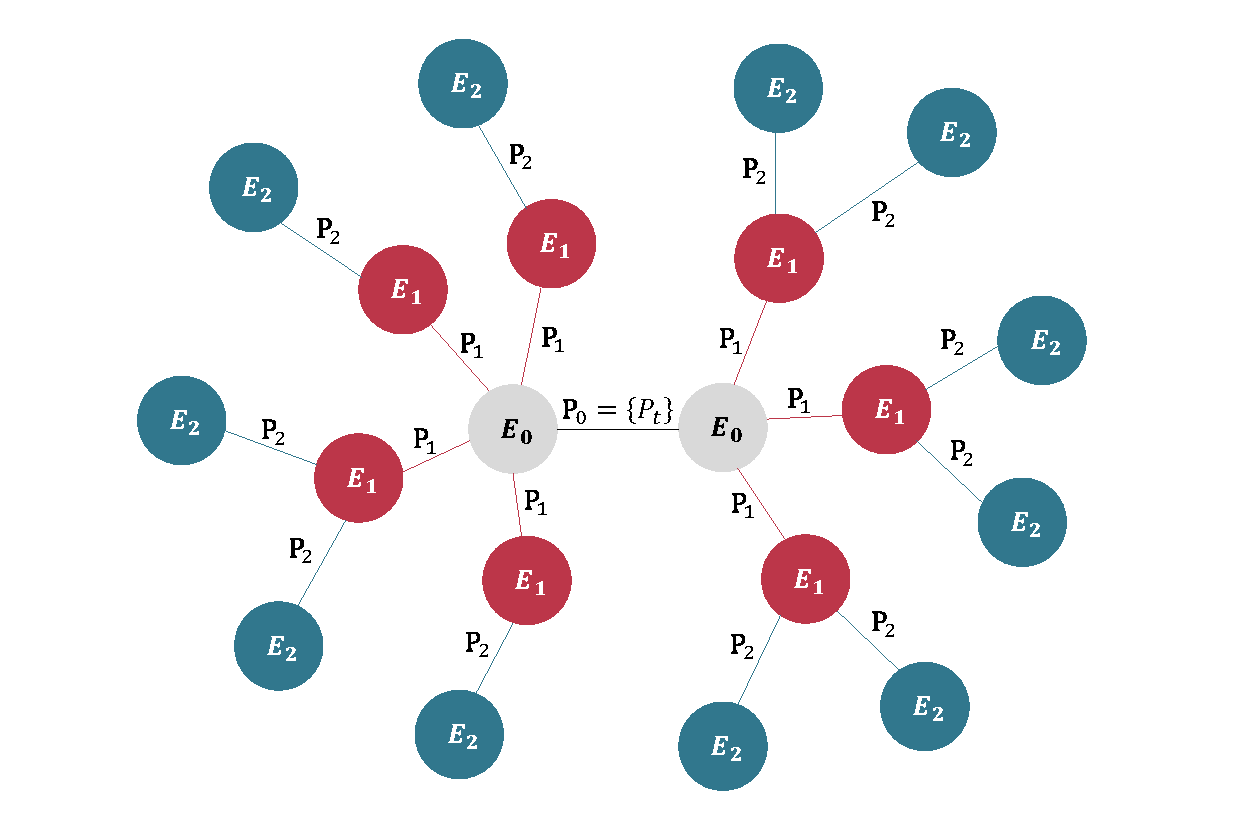
\includegraphics[width=75mm]{sample.pdf}\\
		\caption{Sample for the target predicate $P_t$.}
		\label{fig:sample}
	\end{figure}
	As can be seen from Figure~\ref{fig:sample}, begining with the target predicate $P_t$ (get $P_0$), the related entities are sampled (get $E_0$). Then the sample range of predicates is expanded (get $P_i$) according to the maximum length of the body atoms to obtain the related entities and facts (get $E_i$). 
	
	Assuming the $MaxLen = n$, the incrementing process of the sample is as follows:
	% 去重工作的整理!!
	\begin{itemize}
		\item $K_0=\{E_0, P_0, F_0\}$, where $P_0=\{P_t\}$, \\
		$E_0=\{e | P_t(e, e^{'}) \in F$ or $P_t(e^{'}, e) \in F\}$, \\
		$F_0=\{P_t(e_s,e_o) | P_t(e_s,e_o) \in F \}$.
		\item $K_i=\{E_i, P_i, F_i\}$, $0<i<n$, where \\
		$P_i=\{P|e^{'} \in E_{i-1}, P(e, e^{'})\in F$ or $P(e^{'},e)\in F\}$,\\
		$E_i=\{e|e^{'} \in E_{i-1}, P(e, e^{'})\in F$ or $P(e^{'},e)\in F\}$,\\
		$F_i=\{P(e_s, e_o)|e_s$ or $ e_o \in E_{i-1}, P(e_s, e_o)\in F\}$.
	\end{itemize}
	
	The final sampled $K^{'} = \{E^{'}, P^{'}, F^{'}\}$ is a subset of K, where $E^{'}=\cup^{n-1}_{i=0}E_i$, $P^{'}=\cup^{n-1}_{i=0}P_i$ and $F^{'}=\cup^{n-1}_{i=0}F_i$. 
	% new add!
	Although there must be duplicate predicates in the set $P_i$ at each $i$th layer, it doesn't matter because we allow recursionin the CP rules. In the latter rule search phase, the sequence obtained by performing the Cartesian product operation on the predicate set $P_i$ of each layer can effectively reduce the computation cost compared to using the Cartesian product of all the predicate set$P$.
	In the work of repeating the RLvLR algorithm, we first sample all the entities and predicates of maximum layers, and then perform rule search. In most cases, when the rule length reaches 5 (including head), $P^{'}=P$.
	
	% new add!
	NEW ADD:
	($length$ not include head)
	$$length = 2, P_1\times P_1$$
	$$length = 3, P_1\times P_2\times P_1$$
	$$length = 4, P_1\times P_2\times P_2\times P_1$$
	$$length = 5, P_1\times P_2\times P_3\times P_2\times P_1$$
	$$\cdots$$
	
	\subsection{Embedding Model}
	After sampling, in \textsf{Embedding($\cdot$)}, entities and predicates in $K^{'}$ are embedded into the representation of vector ($ent_{emb}$ and $pre_{emb}$) using the embedding model, respectively. Unlike {\bf RESCAL}, which is used in {\bf RLvLR} to embed predicates as matrices, we use those such that {\bf TransE} can project predicates into vectors.

	The embedding model represents entities and relationships in the knowledge graph, defining a scoring function to learn the continuous representation of entities and relationships. Among the various models, the Translational Distance Model is a outstanding and relatively simple but effective kind of model.
	Given a fact: $P_r(e_h,e_t)$, the {\bf TransE} model represents the relationship as translation vector $\vec{r}$, and the scoring function is defined as: the distance between $\vec{h}+\vec{r}$ and $\vec{t}$: 
	\begin{equation}
	f_r(h, t) = -||\vec{h}+\vec{r} -\vec{t}||_{1/2}
	\label{eq:transe}
	\end{equation}
	When this fact exists in KG, the score $f_r(h,t)$ is higher, i.e. $\vec{h}+\vec{r} \approx \vec{t}$.
	
	The choice of embedding models needs to be considered in conjunction with the methods of calculating the score functions. In the next phase Rule Search, it will be further explained why we choose {\bf TransE}.
	
	\subsection{Simplified Rule Search}
	In the smaller KG $K^{'}$, the task of searching for candidate rules in \textsf{RuleSearch($\cdot$)} is actually
reduced to the search for plausible paths of body predicates. As shown in formula~\ref{eq:cp rule}, the target predicate of the head has been fixed. However, score functions are needed to measure which paths conform to both the form of cp rules and the intrinsic meaning of the rules and further prune for the search space to handle large KGs more efficiently. It was mentioned before that the embedding model was used to map small $K'$ predicates into vectors, so the design of scoring function for embedding calculations would be changed and simplified. 
	
	Let's take the example of a rule with $length=3$, where the predicates of head and body are included:
	\begin{equation}
	P_1(x, z) \wedge P_2(z, y)  \to P_t(x, y). \nonumber
	\end{equation}
	
	\subsubsection{Synonymy Score Function}
	Before we introduce synonymy, we should abstract out the form of CP rules first. The path of predicates in body can be abstracted into a compositional relation $P_{body}$ that approximates target predicate $P_t$ if the rule is reasonable. Therefore, \textit{synonymy} refers to this similar relationship between $P_{body}$ and $P_t$. In {\bf RLvLR} and the work of ~\cite{Yang:2015}, the embedding of compositional relation path is defined as the matrix multiplication of predicates. Here we consider the characteristics of {\bf TransE} and combine the previous methods to compute the synonymy:
	\begin{align}
		f_{syn}(r) = & sim(P_{body},P_t)\\
		= &sim({\bf V}_{P_1} + {\bf V}_{P_2}, {\bf V}_{P_t}) \nonumber\\
		= & exp(-||(({\bf V}_{P_1}+ {\bf V}_{P_2} - {\bf V}_{P_t}||_2) \nonumber
	\end{align}
	
	The geometric meaning of vector addition is to use the Parallelogram Law, and the final sum vector is obtained from the beginning of the first vector to the end of the last vector, which is a more theoretical representation for the embedding of body's path.
	
	Compared to matrix multiplication which has a relatively large amount of calculation with the increase of rule length, the addition of vector itself reduces the complexity of calculation and satisfies the addition commutative law, so the results of the same predicates in different order combinations are the same. For two predicates $P_1$ and $P_2$, we only need to calculate ${\bf V}_{P_1}+{\bf V}_{P_2}$ once, and for matrix multiplication in {\bf RLvLR}, they need to calculate ${\bf M}_{P_1}\cdot {\bf M}_{P_2}$ and ${\bf M}_{P_2}\cdot {\bf M}_{P_1}$ . As the length of rule increases, it will greatly improve scalability when exploring the entire path of search space grows dramatically.

	\subsubsection{Co-occurence Score Function}
	Besides synonymy, co-occurrence is also widely studied in natural language processing~\cite{Jones:Co-occurence}. We can obviously observe a characteristic of the CP rule is that adjacent predicates in the body atoms share the same parametric variables, such as $P_1(x,z)$ sharing variables $z$ with $P_2(z,y)$. It means the rule $r$ is still reasonable when there are large numbers of entities instantiating the parameter $z$. This feature of sharing is called \textit{Co-occurence}. 
	
	The co-occurrence score function we use is the same as the definition of {\bf RLvLR}. It is based on the notion of argument embeddings, the average value of
the embeddings of all the entities appearing in the position of
this argument. Formally, the embeddings of the subject and
object argument of a predicate P are defined as:
	$$
	{\bf V}_P^s = \frac{1}{n} \sum _{e \in E_P^s}k_e.{\bf E} \text{\quad and\quad}	
	{\bf V}_P^o = \frac{1}{n} \sum _{e \in E_P^o}l_e.{\bf E} 
	$$ 
	where $n = \#\{P(e_s, e_o) \in F^{'}\}, E_P^s = \{e_s|\exists e_o \text{ s.t. } P(e_s, e_o)\\
	\in F^{'}\} , E_P^o = \{e_o|\exists e_o \text{ s.t. } P(e_s, e_o) \in F^{'}\}$, $F^{'}$ is defined by\\
	sample phase, $k_e = \#\{P(e, e_o)|\exists e_o \text{ s.t. } P(e, e_o) \in F^{'} \}$ and
$l_e = \#\{P(e_s,e)|\exists e_s \text{ s.t. } P(e_s, e) \in F^{'} \}$. {\bf E} denotes the embedding of $e$.
	
	According to the definition of co-occurrence, the embedding of the object argument of $P_1$ should be similar to the
embedding of the subject argument of $P_2$, denoted ${\bf V}^o_{P_1} \approx {\bf V}^s_{P_2}$.
Similarly, in addition to this, there is a shared relationship between $P_t$ and the body atoms: ${\bf V}^s_{P_1} \approx {\bf V}^s_{P_t}$ and ${\bf V}^o_{P_2} \approx {\bf P}^o_{P_t}$. Thence, the co-occurrence scoring function is defined as follows:
	\begin{align}
	f_{co}(r) = &sim({\bf V}^o_{P_1}, {\bf V}^s_{P_2}) + sim({\bf V}^s_{P_1}, {\bf V}^s_{P_t}) \nonumber\\
	 +& sim({\bf V}^o_{P_2}, {\bf P}^o_{P_t}) 
	\end{align}
	Note that the calculation of $sim$ is similar to that of synonymy.
	
	Finally, after using both of these two scoring functions to complement each other and purne the poor rules, the set of candidates will be saved for the final evaluation.
	

	
	
	\subsection{Evaluate and Filter}
	The candidate rules that are initially screened by the calculated scoring functions are just a set of results that we obtain by some operations. We also need to use the evaluation function \textsf{EvaluateAndFilter($\cdot$) }to check whether these rules meet the expectations of cognition or the actual situation based on the data. Although KGs are still far from completion, it is necessary to ignore these missings or errors in practice. After being evaluatd by differnent levels of degrees in $Degree$, the last remaining rule is relatively high quality.
	Besides, We propose a supervised method of learning the weights of rules, using the TensorLog operation to construct a parametric learning model to achieve the final rule evaluation.

	In the previous related work, like~\cite{Chen:ScaLeKB} ~\cite{Galarraga:AMIE+} and~\cite{Omran:RLvLR}, standard confidence (SC) and head coverage (HC) usually be used for assessing the quality of rule.~\cite{Omran:RLvLR} proposed a efficient method to calculate them in the way of matrix multiplication.
	% need to modify!!!
	In addition to the two degrees,~\cite{Galarraga:AMIE+} also proposed an improved metric based on SC called xx, but it has been proven to not achieve good results.
	
	Suppose $r$ is a CP rule in the form of formular~\ref{eq:cp rule}. The support degree is defined as the nunber of entity pairs which make the  facts, body and head atoms of the rule instantiated with other entities, exist in KG:
	\begin{equation}
		supp(r) = \#\{(e_0, e_n) | P_{body}(e_0, e_n) \land P_t(e_0, e_n)\} \nonumber
	\end{equation}
	where $P_{body}(e_0, e_n)$ means $\exists e_1, \dots, e_{n-1}$ in the KG such that $P_1(e_0, e_1), P_2(e_1, e_2), \dots, P_n(e_{n-1}, e_n)$ exist in the KG. We count the number of entity pairs as support instances.
	
	However, only counting the number of occurrences in KG is not able to fully evaluate this rule. Because KG is incomplete, the frequency of different instances varies greatly. Therefore, the support degree should be calculated for satisfying the probability ratio of body and head respectively, which can better indicate the quality.
	% E.g, add?
	
	So the degrees of standard confidence
(SC) and head coverage (HC) are defined as follows: 
	\begin{align}
		SC(r) =& \frac{supp(r)}{\#(e_0, e_n):body(r)(e_0, e_n)}\\
		HC(r) =& \frac{supp(r)}{\#(e_0, e_n):P_t( e_0, e_n)}
	\end{align}
	% add NSC? A Novel Evaluation Metric.
	
	\subsubsection{The Weight of Rule}  
	In the set of rules for the same target predicate $P_t$, the confidences of distinct rules are different, and the facts obtained by rule with higher weight has higher confidence. Since KGs are incomplete and contain many noisy data, the accuracy of evaluation may be affected by the method of counting accurately the support degree of the rule in KG. Except for the above method, it is also feasible to use the supervised parameter learning model to learn the weight of rules more flexibly. We combine TensorLog operation and one-hot encoding to construct the weight model for the rules of given target predicate $P_t$.
	
	The TensorLog is a method of differentiable probabilistic logic, which has been used for
	probabilistic deductive database in~\cite{Cohen:TensorLog}, KB reasoning in~\cite{Yang:NeuralLP} and so on. Next, we introduce TensorLog operator and then describe how they can be used for weight learning. 
	\begin{align}
		Rule\quad 1: &P_1 \land P_2 \to P_t, w_1\nonumber\\
		Rule\quad 2: &P_3 \land P_4 \to P_t, w_2\nonumber\\
		&\cdots \cdots \nonumber
	\end{align}
	
	For the group of rules about $P_t$, $n$ denotes the number of rules that make $P_t$ as its head predicate, and $w_i$ is the confidence of rule $i$. The loss function of the model is as follows:
	\begin{equation}
		min\sum_{i=1}^{n}\Vert w_i\prod_{k\in p_i}{\bf M}_{P_k}-{\bf M}_{P_t}\Vert_2
		\label{eq:weight model}
	\end{equation}
	
	TensorLog defines an operator $M_P$ for each predicate $P$. Concretely, $M_P$ is the one-hot encoding matrix in $\{0,1\}^{|E| \times|E|}$ such that its $(i,j)$ entry is set 1 if and only if $R(i, j)$ is in the knowledge graph, where $i$ is the $i$-th entity and similarly for $j$. $E$ is the collection of entities about $P_t$ obtained by the sampling algorithm. $p_i$ denotes the path of body atoms of rule $i$ and $R_k$ means the predicate at the $k$th position on the path.
	
	\subsection{Transfer to Uncertain KGs}
	%To be completed.
	Since uncertain knowledge graphs have attracted the attention of more and more researchers, we have tried to transfer the rule learning into the uncertain KGs. In the weight learning model of evaluation phase, we intend to substitute the confidence of triple for the non-zero entries of the matrix.


	\section{Experiments}
	\subsection{Deterministic KGs}
	\subsubsection{Compare with Yang. with FB15k237.}
	\subsubsection{Compare with AMIE+ , Neural LP and RLvLR with DB, Yago2s, Wikidata.}
	% length 更长,侧重效率更高,数量也多
	\subsection{Unceratin KGs}
	\subsubsection{Use NELL and ConceptNet.}
	
	
	\section{Conclusion}
	
	
	\section*{Acknowledgments}
	
	
	%\newpage
	%% The file named.bst is a bibliography style file for BibTeX 0.99c
	\bibliographystyle{named}
	\bibliography{rulelearning}
	
\end{document}